\section{Дослідження розроблених алгоритмів}

\subsection{Дослідження моделі похибок БІНС}

Перевіримо модель та впливи різних складових похимок, на модель БІНС, зобразимо їх в
залежності від часу. Моделювання проведемо над стаціонарно закріпленою БІНС.
Для початку перевіримо випадок коли координатний трьохгранник має невеликий нахил,
помилку $\Delta \alpha_{E}$. Це призведе до того, що на горизонтальний акселерометр
подіє прискорення $-g \alpha_{E}$. Виміряне прискорення спричинить, до того, що після
двох інтеграторів, буде здаватись, що система має швидкість і відповідно рухається.
Це спричинить момент на гіроскопах в напрямку зменшення зміщення помилки
координатного трьох гранника, але коли акселерометр стає зрівноваженим система 
матиме значну швидкість, що продовжить коливання. Це нагадує маятник, коли відхиляють
підвіс і дають йому коливатись

\begin{figure}[here]
\centering
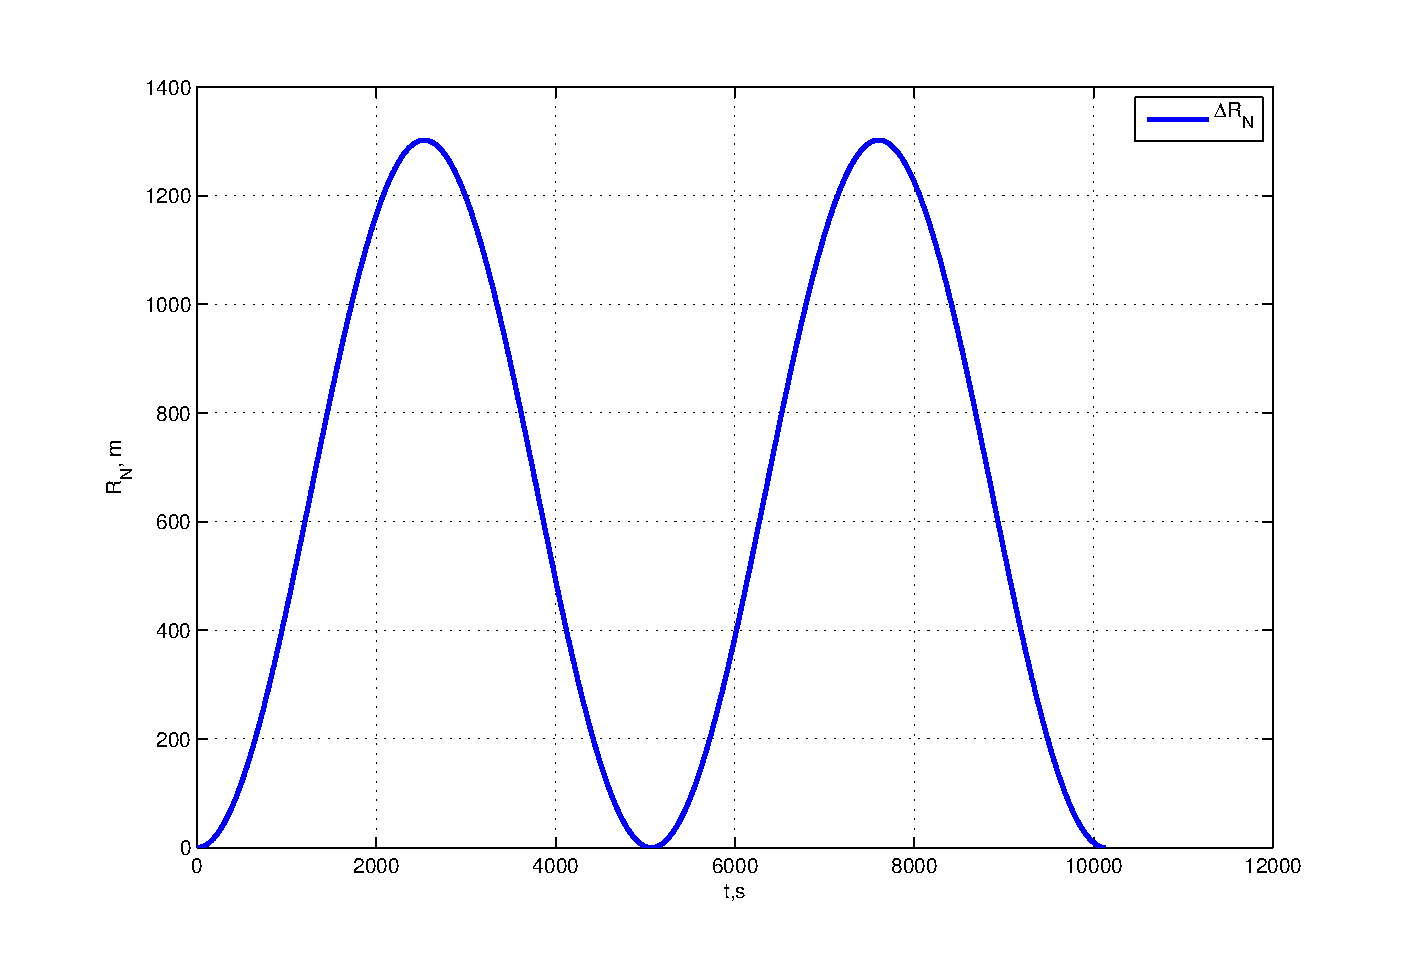
\includegraphics[scale=0.4]{ins_stat_tilt}
\caption{Еволюція похибки за умови, похибки координатного тригранника $10^{-3} rad$}
\label{fig:ins_stat_tilt}
\end{figure}

На рис. \ref{fig:ins_stat_tilt} зображено результат моделювання руху похибки ІНС
яка зумовлена початковим зміщенням координатного тригранника на $10^{-3} rad$.
Можна зазначити, що помилка коливається з частотою Шулера, з періодом 84.4 хвилини.
Найбільша помилка приблизно 1300 метрів і досягається приблизно за 42.2 хвилини роботи системи.

Розглянемо еволюцію похибок при наявності дрейфа гіроскопа. Ефект дрейфа гіроскопа позначається на нахилі координатного тригранника, в результаті виникає помилка прискорення. Швидкість і координата коливаються з частотою Шулера. Але цього разу швидкість
коливається не навколо нуля, отже помилка координати утворюється як сума лінійної наростаючої та гармонічної функції.

 Яскраво виражені коливання Шулера та лінійно наростаюча функція на рис.\ref{fig:ins_stat_gyro} як загальна помилка для стаціонарно закріпленої ІНС з дрейфом вертикального гіроскопа на $0.01^{o}/h$,. Після 1 години роботи похибка по координаті приблизно 1300 метрів. Якщо гіроскоп менш точний то його дрейф спричиняє похибку 1600 метрів за 10 хвилин. Зрозуміло, що на не дорогих ДПІ похибка зростає до 1500 метрів за 1 хвилину.
\begin{figure}[here]
\centering
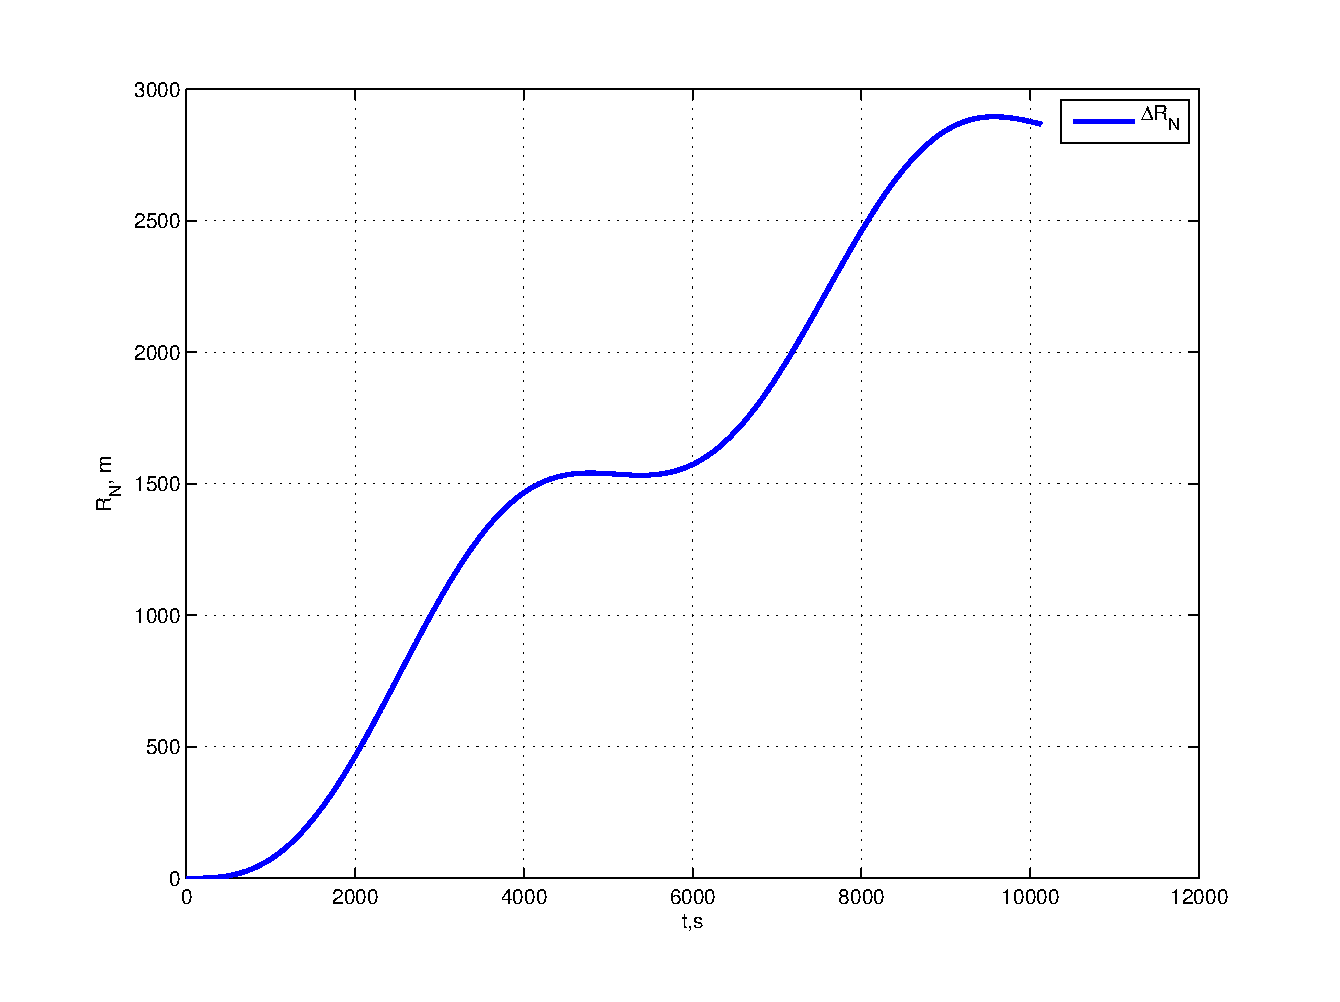
\includegraphics[scale=0.4]{ins_stat_gyro}
\caption{Еволюція похибки за умови, дрейфу гіроскопа $0.01 deg/h$}
\label{fig:ins_stat_gyro}
\end{figure}

При наявності помилки по швидкості $\Delta V_{E} =1$ м/с позиційна похибка буде обмеженою і коливатиметься з частотою Шулера рис.\ref{fig:ins_stat_velo}.
\begin{figure}[here]
\centering
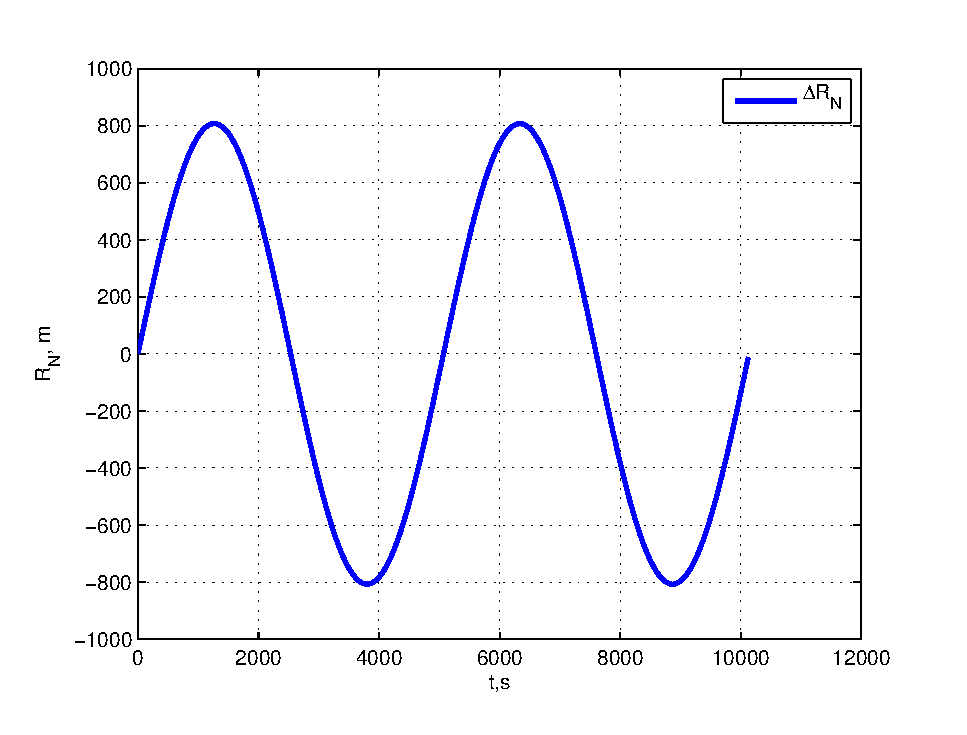
\includegraphics[scale=0.5]{ins_stat_velo}
\caption{Еволюція похибки при початковій похибці по швидкості 1 м/с}
\label{fig:ins_stat_velo}
\end{figure}

Далі порівняємо ефект впливу помилок різного типу в стаціонарно закріпленій ІНС. На рис. \ref{fig:ins_stat_sum}.
На малюнку зображено вплив кожного виду помилки: помилку початкової виставки як помилку нахилу координатного тригранника та помилки ДПІ як дрейфи акселерометра та гіроскопа. Також результуючу помилку по координаті, як суму перерахованих вище.
\begin{figure}[here]
\centering
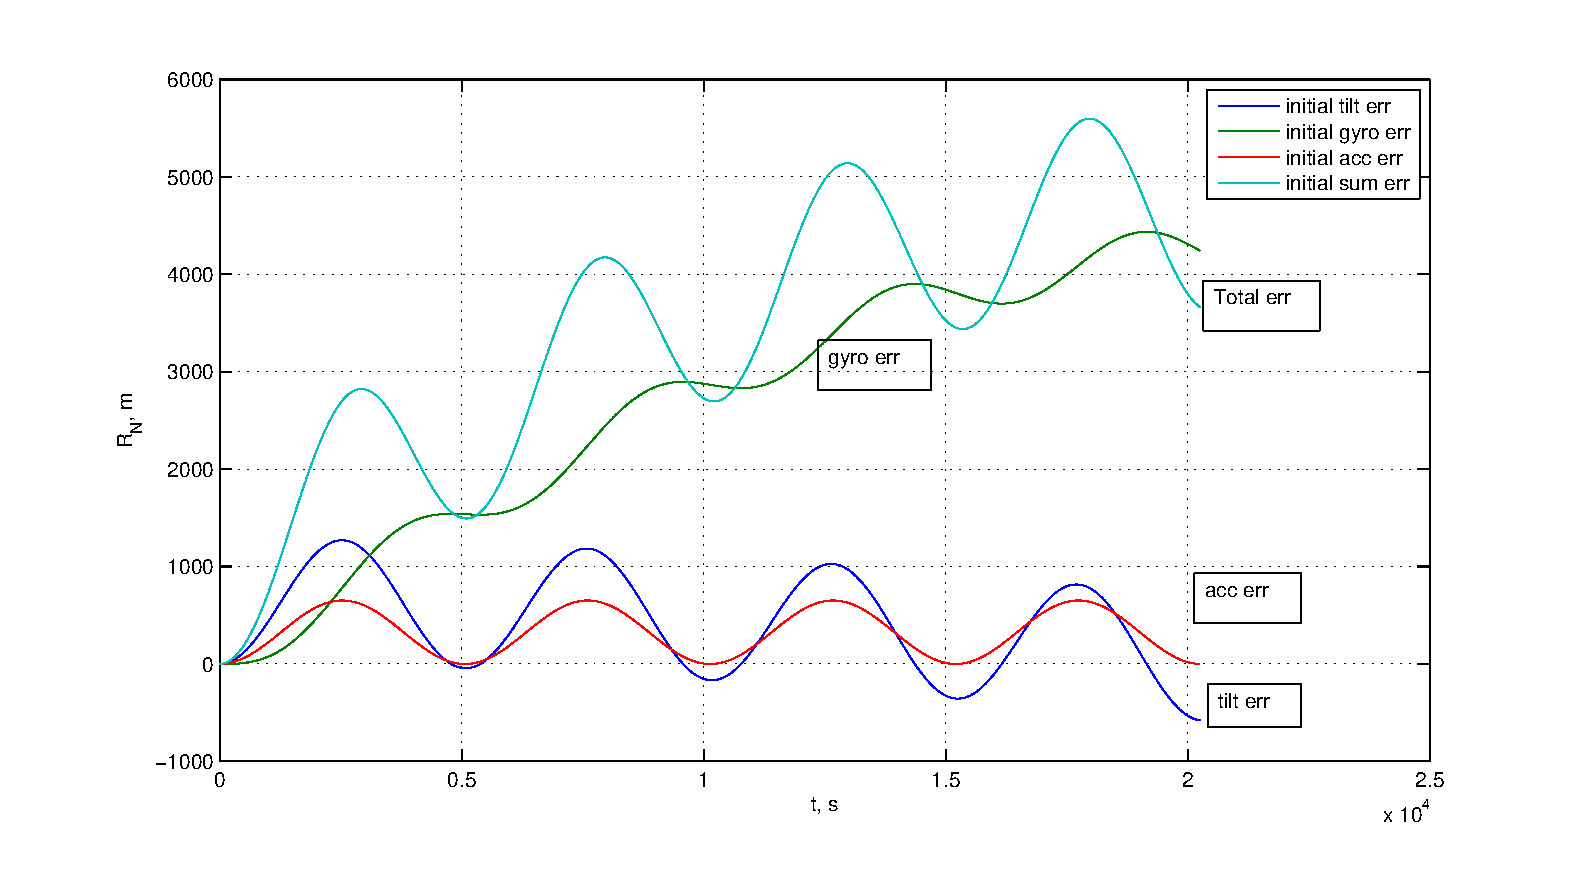
\includegraphics[scale=0.67]{ins_stat_sum}
\caption{Еволюція сумарної похибки по координаті за умови,
дрейфу гіроскопа   $0.01 deg/h$,похибки координатного тригранника $10^{-3} rad$, та зміщенням акселерометра $10^{-4} rad$ }\label{fig:ins_stat_sum}
\end{figure}

Можна зауважити, що за виключенням початкової виставки, сумарна похибка по координаті переважно визначається дрейфом гіроскопа. Дрейф інтегрується один раз, коли розраховується кут для перетворення прискорення, який потім інтегрується вдруге для отримання позиційної похибки.

\subsection{Рівняння траєкторії ЛА}


